\section{Results on TabReD: how far architecture carries a weak model}
\label{sec:ceiling}

% STAGE 3: rewritten 8 September 2026.  Every number is a macro from
% tables/numbers.tex unless it has no source in make_tables.py.

This section answers RQ1 and RQ2 on the eight TabReD tasks.
Figure~\ref{fig:ranks} places the three systems among the eighteen published
methods, task by task in the benchmark's own metrics and, on top, by average
rank. Table~\ref{tab:leaderboard} gives the raw values. The text below also
uses the normalised score of Section~\ref{sec:benchmarks}, on which $0$ is the
weakest and $1$ the strongest published method on each task.

\begin{figure*}[t]
\centering
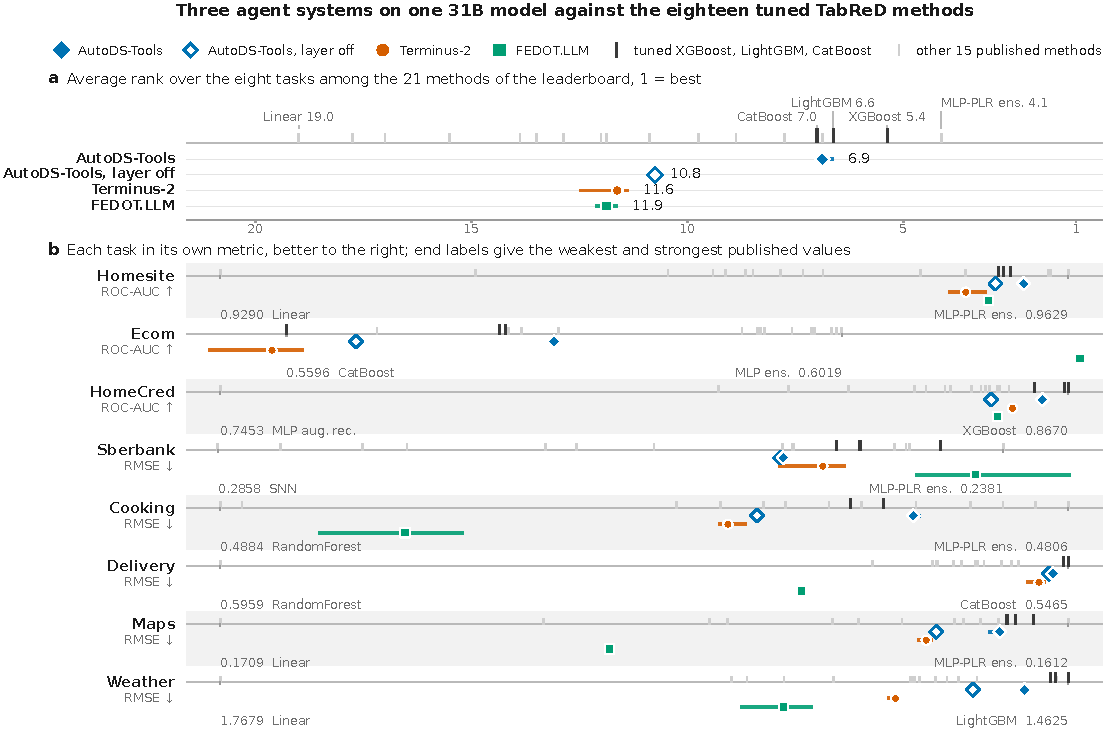
\includegraphics[width=\textwidth]{figures/fig_ranks.pdf}
\caption{The three systems among the eighteen tuned TabReD methods. (a)~Average rank over the eight tasks among the \nMethods{} methods of Table~\ref{tab:leaderboard}; whiskers span the average rank of the best and worst attempts. (b)~One strip per task in the task's own metric, better to the right; ticks are the published methods, the darker three the tuned gradient-boosting methods, the end labels the weakest and strongest published values. Rows within a task: AutoDS-Tools with the layer on (filled) and off (open), Terminus-2, FEDOT.LLM; whiskers span three attempts.}
\label{fig:ranks}
\end{figure*}
\begin{table*}[t]
\centering
\caption{Agent architectures placed in the TabReD leaderboard: full official temporal splits, the benchmark's metrics in raw units. Published rows are Optuna-tuned means over 15 seeds \citep{rubachev2024tabred}; agent rows use \texttt{gemma-4-31b-it}; agent rows are means over three attempts. Best per column in bold.}
\label{tab:leaderboard}
\small
\setlength{\tabcolsep}{3pt}
\begin{tabular}{lrrrrrrrrr}
\toprule
& \multicolumn{3}{c}{ROC-AUC $\uparrow$} & \multicolumn{5}{c}{RMSE $\downarrow$} & \\
\cmidrule(lr){2-4}\cmidrule(lr){5-9}
Method & Homesite & Ecom & HomeCred & Sberbank & Cooking & Delivery & Maps & Weather & Avg.\ rank \\
\midrule
\addlinespace[2pt]
\multicolumn{10}{l}{\itshape GBDT} \\
XGBoost & 0.9601 & 0.5763 & \textbf{0.8670} & 0.2419 & 0.4823 & 0.5468 & 0.1616 & 1.4671 & 5.4 \\
LightGBM & 0.9603 & 0.5758 & 0.8664 & 0.2468 & 0.4826 & 0.5468 & 0.1618 & \textbf{1.4625} & 6.6 \\
CatBoost & 0.9606 & 0.5596 & 0.8621 & 0.2482 & 0.4823 & \textbf{0.5465} & 0.1619 & 1.4688 & 7.0 \\
RandomForest & 0.9570 & 0.5764 & 0.8269 & 0.2640 & 0.4884 & 0.5959 & 0.1653 & 1.5838 & 17.8 \\
Linear & 0.9290 & 0.5665 & 0.8168 & 0.2509 & 0.4882 & 0.5579 & 0.1709 & 1.7679 & 19.0 \\
\addlinespace[2pt]
\multicolumn{10}{l}{\itshape Tabular DL} \\
MLP & 0.9500 & 0.6015 & 0.8545 & 0.2508 & 0.4820 & 0.5504 & 0.1622 & 1.5470 & 9.8 \\
SNN & 0.9492 & 0.5996 & 0.8551 & 0.2858 & 0.4838 & 0.5544 & 0.1651 & 1.5649 & 15.5 \\
DCNv2 & 0.9392 & 0.5955 & 0.8466 & 0.2770 & 0.4842 & 0.5532 & 0.1672 & 1.5782 & 17.0 \\
ResNet & 0.9469 & 0.5998 & 0.8493 & 0.2743 & 0.4825 & 0.5527 & 0.1625 & 1.5021 & 12.0 \\
FT-Transformer & 0.9622 & 0.5775 & 0.8571 & 0.2440 & 0.4820 & 0.5542 & 0.1625 & 1.5104 & 8.9 \\
MLP (PLR) & 0.9621 & 0.5957 & 0.8568 & 0.2438 & 0.4812 & 0.5527 & 0.1616 & 1.5177 & 6.9 \\
Trompt & 0.9588 & 0.5803 & 0.8355 & 0.2509 & 0.4809 & 0.5519 & 0.1624 & 1.5187 & 10.9 \\
\addlinespace[2pt]
\multicolumn{10}{l}{\itshape Ensembles} \\
MLP ens. & 0.9503 & 0.6019 & 0.8557 & 0.2447 & 0.4815 & 0.5494 & 0.1620 & 1.5186 & 7.8 \\
MLP-PLR ens. & \textbf{0.9629} & 0.5981 & 0.8585 & \textbf{0.2381} & \textbf{0.4806} & 0.5518 & \textbf{0.1612} & 1.4953 & 4.1 \\
\addlinespace[2pt]
\multicolumn{10}{l}{\itshape Training methodologies} \\
MLP aug. & 0.9523 & 0.6011 & 0.8449 & 0.2659 & 0.4832 & 0.5532 & 0.1631 & 1.5193 & 13.5 \\
MLP aug. rec. & 0.9531 & 0.5960 & 0.7453 & 0.2515 & 0.4834 & 0.5541 & 0.1636 & 1.5160 & 13.9 \\
\addlinespace[2pt]
\multicolumn{10}{l}{\itshape Retrieval-augmented} \\
TabR & 0.9487 & 0.5943 & 0.8501 & 0.2820 & 0.4828 & 0.5514 & 0.1639 & 1.4666 & 12.9 \\
ModernNCA & 0.9514 & 0.5765 & 0.8531 & 0.2593 & 0.4825 & 0.5498 & 0.1625 & 1.5062 & 11.9 \\
\midrule
\multicolumn{10}{l}{\itshape Agentic AutoML systems (this work)} \\
Terminus-2 \emph{(open harness)} & 0.9588 & 0.5585 & 0.8590 & 0.2491 & 0.4837 & 0.5482 & 0.1628 & 1.5247 & 11.6 \\
AutoDS-Tools \emph{(multi-agent)} & 0.9611 & 0.5800 & 0.8633 & 0.2515 & 0.4820 & 0.5474 & 0.1620 & 1.4783 & 6.9 \\
FEDOT.LLM \emph{(rigid pipeline)} & 0.9597 & \textbf{0.6200} & 0.8569 & 0.2398 & 0.4867 & 0.5620 & 0.1664 & 1.5651 & 11.9 \\
\bottomrule
\end{tabular}
\end{table*}


\subsection{The best system reaches tuned LightGBM and no system reaches tuned XGBoost}
\label{sec:halfrange}

With the backbone fixed, the three systems as deployed span $\spanShip$ on
the normalised scale: AutoDS-Tools $\nAutoDS$, FEDOT.LLM $\nFedot$ and
Terminus-2 $\nTerminus$ (Figure~\ref{fig:ranks}). In average rank over the
\nMethods{} methods of Table~\ref{tab:leaderboard} the order reads
$\rkAutoDS$, $\rkFedot$ and $\rkTerminus$, the last two level. Most of the
spread belongs to the prescribed-knowledge layer: without it AutoDS-Tools
scores $\nAutoDSOff$, and the three architectures then lie within $\spanArch$
of each other, of the same order as the run-to-run noise of
Section~\ref{sec:design}. We quote $\spanArch$ whenever the claim is about
architecture and $\spanShip$ only when the systems are compared as deployed.

The best system does not reach tuned practice. Tuned XGBoost sits at $\nXGB$
(rank $\rkXGB$) and the strongest published method at $\nBest$ (rank
$\rkBest$). AutoDS-Tools at $\nAutoDS$ sits among the three tuned
gradient-boosting methods, level with LightGBM at $\nLGBM$, ahead of CatBoost
at $\nCat$ and $\gapXGB$ below XGBoost, and no architecture approaches the
strongest published method. Against default configurations, the comparison
most papers make, the same systems would appear to win outright.

FEDOT.LLM sits between the two agentic systems on the normalised mean and
level with Terminus-2 in average rank, and the two readings differ for one
reason. On \texttt{ecom-offers} its tuned stack of logistic regression,
CatBoost, XGBoost and LightGBM reaches ROC-AUC $\fedotEcomAuc$, above every
published method ($\nFedotEcom$ on a scale where the strongest published
method is $1$); without that task it scores $\nFedotNoEcom$ against
$\nTerminusNoEcom$ for Terminus-2 and $\nAutoDSNoEcom$ for AutoDS-Tools,
last of the three. It is the only system in the comparison that searches over
its models: the same stack on the other two classification tasks, a random
forest or LightGBM regressor on the regression tasks, tuned within a
$1200$\,s backend budget (Section~\ref{sec:deviations}). The search costs
time: $\minFedotTabredMin$ to $\minFedotTabredMax$ minutes a task against
$\termMedianMin$ at the median for Terminus-2 (Section~\ref{sec:cost}).

\paragraph{Observation 1} With one open 31B backbone, the three systems as
deployed span $\spanShip$ on the normalised scale, and with the AutoDS-Tools
layer removed the three architectures lie within $\spanArch$. With the layer
on, AutoDS-Tools reaches $\nAutoDS$: level with tuned LightGBM, ahead of tuned
CatBoost, and $\gapXGB$ short of tuned XGBoost.

\subsection{The prescribed-knowledge layer separates the two agentic systems}
\label{sec:grid}

The deployed configurations differ in more than architecture. AutoDS-Tools
carries its prescribed-knowledge layer and runs on an image provisioned with
the libraries that layer names, while Terminus-2 receives the task statement
alone on the stock image. Provisioning alone changes nothing
(Section~\ref{sec:matched}); the layer accounts for most of the distance.
With the layer removed, the \emph{untreated} cell of Table~\ref{tab:grid} on
the same tasks and image, AutoDS-Tools scores $\nAutoDSOff$ against
$\nAutoDS$ as deployed: its margin over Terminus-2 shrinks from
$\gapAgentsShip$ to $\gapAgentsOff$, so the layer accounts for
$\layerWorthNorm$ of the $\gapAgentsShip$ and the architecture for
$\gapAgentsOff$, and AutoDS-Tools falls $\fedotAboveAutoDSOff$ below
FEDOT.LLM.

\begin{table*}[t]
\centering
\caption{The prescribed-knowledge layer split into its halves on AutoDS-Tools over TabReD, twenty-four trials per cell on one image and one machine. The untreated cell is given in the task's own units; the other three as relative change against it, positive is better.}
\label{tab:grid}
\small
\setlength{\tabcolsep}{5pt}
\begin{tabular}{llrrrr}
\toprule
 & & untreated & \multicolumn{3}{c}{change against untreated, \%} \\
\cmidrule(l){4-6}
Task & Metric & cell & $K_{\text{tool}}$ only & $K_{\text{disc}}$ only & both \\
\midrule
\texttt{homesite-insurance} & ROC-AUC & 0.9600 & +0.10 & -0.03 & +0.12 \\
\texttt{ecom-offers} & ROC-AUC & 0.5649 & +3.68 & +1.24 & +2.67 \\
\texttt{homecredit-default} & ROC-AUC & 0.8559 & +0.79 & +0.20 & +0.86 \\
\texttt{sberbank-housing} & RMSE & 0.2516 & -0.31 & 0.00 & +0.07 \\
\texttt{cooking-time} & RMSE & 0.4835 & +0.47 & -0.04 & +0.30 \\
\texttt{delivery-eta} & RMSE & 0.5476 & 0.00 & -0.05 & +0.04 \\
\texttt{maps-routing} & RMSE & 0.1627 & +0.64 & +0.09 & +0.45 \\
\texttt{weather} & RMSE & 1.4968 & +0.14 & -0.41 & +1.24 \\
\midrule
mean over tasks & & & +0.69 & +0.12 & +0.72 \\
tasks improved & & & 6 of 8 & 3 of 8 & 8 of 8 \\
\bottomrule
\end{tabular}
\end{table*}


On TabReD the two halves of the layer can be switched separately, and
Table~\ref{tab:grid} crosses them: four cells of twenty-four trials on one
image, one machine and one concurrency setting, differing in the instruction
file and in nothing else. Both halves together beat the untreated cell on all
eight tasks, so on this family the layer does no harm. Averaged over the eight tasks, naming the library (\Ktool{}) improves the
metric by $\gridToolMean\%$, prescribing the training discipline (\Kdisc{}) by
$\gridDiscMean\%$, and both together by $\gridBothMean\%$, below the
$\gridSumHalves\%$ sum of the two (interaction $\gridInteraction\%$). The
library instruction carries the effect, and two tasks carry most of it
(Table~\ref{tab:grid}): \texttt{ecom-offers} moves $\gridToolEcom\%$ under
the library half alone and \texttt{homecredit-default}
$\gridToolHomecredit\%$; no other task moves by more than
$\gridToolRestMax\%$.

The two halves also cost differently. Naming a library shortens the agent's
search and lengthens its fitting: the median trial goes from $\gridNeitherMin$
minutes untreated to $\gridToolMin$ with the library named, while the bill per
trial falls from $\gridNeitherCost$ to $\gridToolCost$ dollars. Prescribing
discipline does the opposite, adding $\gridDiscCostPct\%$ to the bill and
cutting the median trial to $\gridDiscMin$ minutes.

\paragraph{Observation 2} As deployed, AutoDS-Tools leads Terminus-2 by
$\gapAgentsShip$ on the normalised scale. Of that, $\layerWorthNorm$ comes from
the prescribed-knowledge layer and $\gapAgentsOff$ from the architecture, so with
the layer off AutoDS-Tools stays ahead by $\gapAgentsOff$. Inside the layer, the library half carries almost the whole
effect and the two halves are non-additive.

\subsection{Provisioning alone does nothing}
\label{sec:matched}

Running Terminus-2 on the image built for AutoDS-Tools, same eight tasks and
three attempts each, leaves \matchedWithin{} of the eight tasks inside the
system's own noise floor, and several attempts reproduce the stock-image
value to every digit. The traces explain why: across all twenty-four trials
the agent named none of the three libraries the enriched image pre-installs
and went to gradient boosting by hand, as on the stock image, where it had
installed the library itself. The enriched image was also defective
(Section~\ref{sec:deviations}), lacking the OpenMP runtime LightGBM links
against; forty-five trials across the two systems met the error, and
forty-five diagnosed it, installed the runtime and continued. Agents rebuild
the environment they need, so installing a library in advance changes only the
container. The one exception is \texttt{sberbank-housing}, at
$\matchedSberbank\%$ with a standard deviation of $\matchedSberbankSD$ RMSE
over three attempts: one attempt trained a thousand boosting rounds without
early stopping, a lapse of the agent (Section~\ref{sec:spontaneous}).

\subsection{A different backbone moves reliability and cost while accuracy holds}
\label{sec:modelaxis}

Figure~\ref{fig:modelaxis} varies the backbone
under both agentic systems, one model smaller of the same generation and one
stronger from another family, with tasks, image, concurrency and machine
unchanged; each system keeps its shipped instruction, AutoDS-Tools with the
layer on and Terminus-2 with the task text alone. Accuracy barely moves. The median change against each system's own
reference row is $\axTerminusSmallDelta\%$ and $\axTerminusBigDelta\%$ for
Terminus-2 and $\axAutoDSSmallDelta\%$ and $\axAutoDSBigDelta\%$ for
AutoDS-Tools, against a bill that varies \axPriceSpread$\times$ across the same
rows. On \texttt{cooking-time} two backbones under Terminus-2 produced
predictions identical to sixteen digits while deliberating differently, and
both ended at the same LightGBM call with the same defaults.

\begin{figure*}[t]
\centering
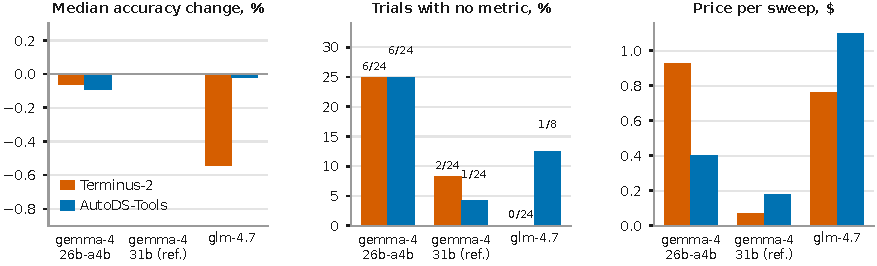
\includegraphics[width=\textwidth]{figures/fig_modelaxis.pdf}
\caption{Swapping the backbone under each architecture on TabReD, everything else fixed. Left: median relative change in the task metric against that system's \texttt{gemma-4-31b} row over trials that returned a metric, positive is better. Middle: trials that returned no metric, labelled as lost over run. Right: price of the whole sweep of twenty-four trials; the upper AutoDS-Tools cell is eight trials, one per task. The per-cell table is in the supplementary material.}
\label{fig:modelaxis}
\end{figure*}

On the normalised scale, replacing the backbone moves the mean score by up to
0.04 under AutoDS-Tools and by up to 0.24 under Terminus-2. The 0.24 comes
from one task: \texttt{sberbank-housing} alone moves the mean by $0.30$, and
the other seven tasks together move it the other way by $0.07$. For
comparison, the instruction file of AutoDS-Tools moves the mean by
$\layerWorthNorm$, the three architectures without that file differ by
$\spanArch$, and the systems as deployed by $\spanShip$. Under AutoDS-Tools
the instruction file therefore matters more than a backbone
\axPriceSpread$\times$ the price; under Terminus-2 the backbone matters more
than any change of architecture, and through one task. Where accuracy does
move, the cause is the same in both directions: a stronger
backbone more often chooses a model other than the gradient-boosting default. On
\texttt{ecom-offers} that departure produced the best ROC-AUC in this paper,
$0.627$ against $0.554$ to $0.569$ for the reference model; on
\texttt{sberbank-housing} the same departure, to a random forest, cost $46\%$
of RMSE. Prescription and backbone both act on one decision, whether the agent keeps the
gradient-boosting default or overrides it, and the sign of the outcome depends
on whether that default suited the task.

Reliability separates the two systems, in opposite directions. Under
Terminus-2 the trials returning no metric fall from \axTerminusSmallLost{} of
twenty-four to \axTerminusRefLost{} to \axTerminusBigLost{} as the backbone
strengthens. Under AutoDS-Tools they are lowest at the model the system was
built against, \axAutoDSRefLost{} of twenty-four, and rise on both sides, to
\axAutoDSSmallLost{} of twenty-four below it and \axAutoDSBigLost{} of the
\axAutoDSBigTrials{} trials we could afford above it; trials cut at the time
limit move the same way, at \axAutoDSRefCutPct{}, \axAutoDSSmallCutPct{} and
\axAutoDSBigCutPct{} per cent. A stronger model makes the six agents exchange
more text inside the same hour, so more trials reach the time limit and
accuracy is unchanged. The loss rate is partly a property of the deployment:
the same reference model lost \axTerminusRefLost{} trials of twenty-four here
and none in the matched arm of Section~\ref{sec:matched}, on a different
machine at half the concurrency, so only comparisons within one deployment
are safe.

The backbone comparison has a lower limit. Two models one generation
older, \texttt{gemma-3-12b-it} and \texttt{gemma-3-27b-it}, returned nothing
usable in smoke trials on \texttt{cooking-time}: the smaller emitted tool
calls with empty arguments, the larger wrote a working pipeline and left its
submission in the wrong directory. Below some level of capability a backbone
returns no usable submission, and that level is higher than the parameter
count alone would suggest.

\paragraph{Observation 3} Provisioning the image with libraries that no
instruction names changes nothing measurable. Swapping the backbone across a
\axPriceSpread$\times$ price range moves accuracy by a fraction of a percent. The same swap moves reliability and cost in
opposite directions for the two architectures.

\subsection{Cost: the binding budget is wall-clock}
\label{sec:cost}

\begin{table}[!t]
\centering
\caption{Cost and wall-clock per trial from the Harbor telemetry: means over trials of the trials' own cost, tokens and time. MLAB abbreviates MLAgentBench. Bold: the lowest value in its column within a benchmark.}
\label{tab:cost}
\scriptsize
\setlength{\tabcolsep}{2.5pt}
\begin{tabular}{llrrrrr}
\toprule
System & Bench & $n$ & \$/tr. & In/tr. & Out/tr. & Min/tr. \\
\midrule
Terminus-2 & TabReD & 24 & 0.0069 & 49\,969 & 2\,111 & \textbf{5.1} \\
AutoDS & TabReD & 24 & 0.0074 & 61\,606 & 5\,349 & 44.4 \\
FEDOT.LLM & TabReD & 24 & \textbf{0.0003} & \textbf{2\,680} & \textbf{155} & 33.1 \\
AutoDS ($K$ off) & MLAB & 30 & \textbf{0.0089} & \textbf{76\,463} & \textbf{5\,864} & 63.2 \\
AutoDS (shipped $K$) & MLAB & 30 & 0.0103 & 90\,439 & 6\,407 & 70.5 \\
Terminus-2 & MLAB & 24 & 0.4317 & 1\,989\,443 & 11\,873 & \textbf{19.1} \\
\bottomrule
\end{tabular}
\begin{tablenotes}\footnotesize
\item Distributions are right-tailed: the untreated AutoDS-Tools branch on MLAgentBench has a median of $10.9$ minutes against a mean of $63.2$, and one Terminus-2 trial (\texttt{feedback}, $571$ steps, \$8.71) is $84\%$ of its job, whose median trial cost \$0.033. FEDOT.LLM calls the model from inside its container, so its cost is its token count at list price.
\end{tablenotes}
\end{table}


Token spend does not bind at this scale. In the telemetry of
Table~\ref{tab:cost} a whole TabReD trial costs under a cent for any system,
$\costTerminusTabred$ dollars for Terminus-2, $\costAutoDSTabred$ for
AutoDS-Tools and $\costFedotTabred$ for FEDOT.LLM, whose model calls are a few
thousand tokens a trial and whose $\minFedotTabred$ minutes a trial are
backend search. On the same data adapter AutoDS-Tools spends
$\costRatioDollars\times$ the dollars of Terminus-2, $\costRatioOut\times$
its output tokens and $\costRatioMin\times$ its wall-clock: the money is
negligible, the clock is not.

The price of the layer is read off the crossed cells of Section~\ref{sec:grid}:
the bill falls from $\gridNeitherCost$ to $\gridBothCost$ dollars a trial while
the median trial rises from $\gridNeitherMin$ to $\gridBothMin$ minutes. Naming
a library shortens the search and lengthens the fit, so the sign of its cost
depends on which resource is counted.

What binds is the clock. In the re-run of AutoDS-Tools, twenty-four trials
under the benchmark's own one-hour ceiling, agent wall-clock had a median of
$\rerunMedianMin$ minutes and a minimum of $\rerunMinMin$;
\rerunNearCeiling{} trials finished within fifteen minutes of the ceiling and
\rerunCut{} more were cut by it, of which \rerunCutScored{} had already written
a submission and are scored like any other and \rerunLost{} had not.
Terminus-2 on the same tasks and ceiling has a median of $\termMedianMin$
minutes and a maximum of $\termMaxMin$ per trial. The lost trial is excluded
from the mean, because a timeout measures the budget and says nothing about
the model (Section~\ref{sec:threats}); a second run of the arm on another
machine at half the concurrency gave a median of $37.4$ minutes and two lost
trials.

\paragraph{Observation 4} AutoDS-Tools pays for its accuracy in time: on the
same data adapter it spends $\costRatioMin\times$ the wall-clock of
Terminus-2 for $\costRatioDollars\times$ the money, and \rerunCut{} of its
twenty-four trials run into the one-hour task ceiling.
